\section{The Milestones Project}\label{sec:project}
An early overview of the content and aims of the Milestones Project appeared in \cite{Friendly:04:gfkl}.
Here we update that description and provide a few technical details on some problems in
documenting the history of data visualization in a convenient form for browsing, searching and
analysis.

\subsection{Origin, structure and evolution}\label{sec:structure}
The initial step in portraying the history of data visualization was a simple chronological listing of milestone items
with capsule descriptions, bibliographic references, markers for date, person, place, and links to portraits, images,
related sources or more detailed commentaries.
We started with 105
developments listed by \citet{BenigerRobyn:1978}
and incorporated additional listings from
\citet{Hankins:1999},  \citet{Tufte:1983,Tufte:1990,Tufte:1997},  \citet{Heiser:2000}, and others.

This began as single \LaTeX\ file (with markup tags for all relevant bits of information),
used to produce a
hyper-linked PDF document.  A variety of software tools (perl scripts, Unix utilities) allowed us to turn this
single source
\emph{directly} into the web version originally shown at
\url{http://www.math.yorku.ca/SCS/Gallery/milestone}.  Other custom software tools allowed us to
add new milestones items from text files using a template of tags (DATE:, AUTHOR:, WHAT:, REF:, IMG:, etc.)
and extract the
information about milestones items, authors, images, etc. in a variety of forms (CSV, XML, JSON)
that could be used as input for analyses and graphic displays.  For example, \figref{fig:mileyears4}
was produced in SAS software using a unix command pipe like
\begin{verbatim}
itemdb -o milestones.csv < milestones.tex | sas -i milestones.csv mileyears.sas
\end{verbatim}

\begin{figure}[!htb]
  \centering
  \includegraphics[width=\textwidth,clip]{fig/datavis-timeline2}
  \caption{Timeline view of the Milestones Project on the site \texttt{http://datavis.ca}. In this view,
  the top panel shows a detailed view of the segment of history highlighted in the bottom panel, both
  of which can be separately scrolled. Items in the top panel show a brief tag, color-coded in coarse
  categories. Clicking on an item in this panel brings up small description, linked to the details of
  the milestone item.
  }
  \label{fig:datavis-timeline2}
\end{figure}

It soon became apparent that such a text-based representation was inadequate.  Around 2005, we began
to convert this to a true database and
completely redesigned the Milestones web site. ...

\begin{figure}[!htb]
  \centering
  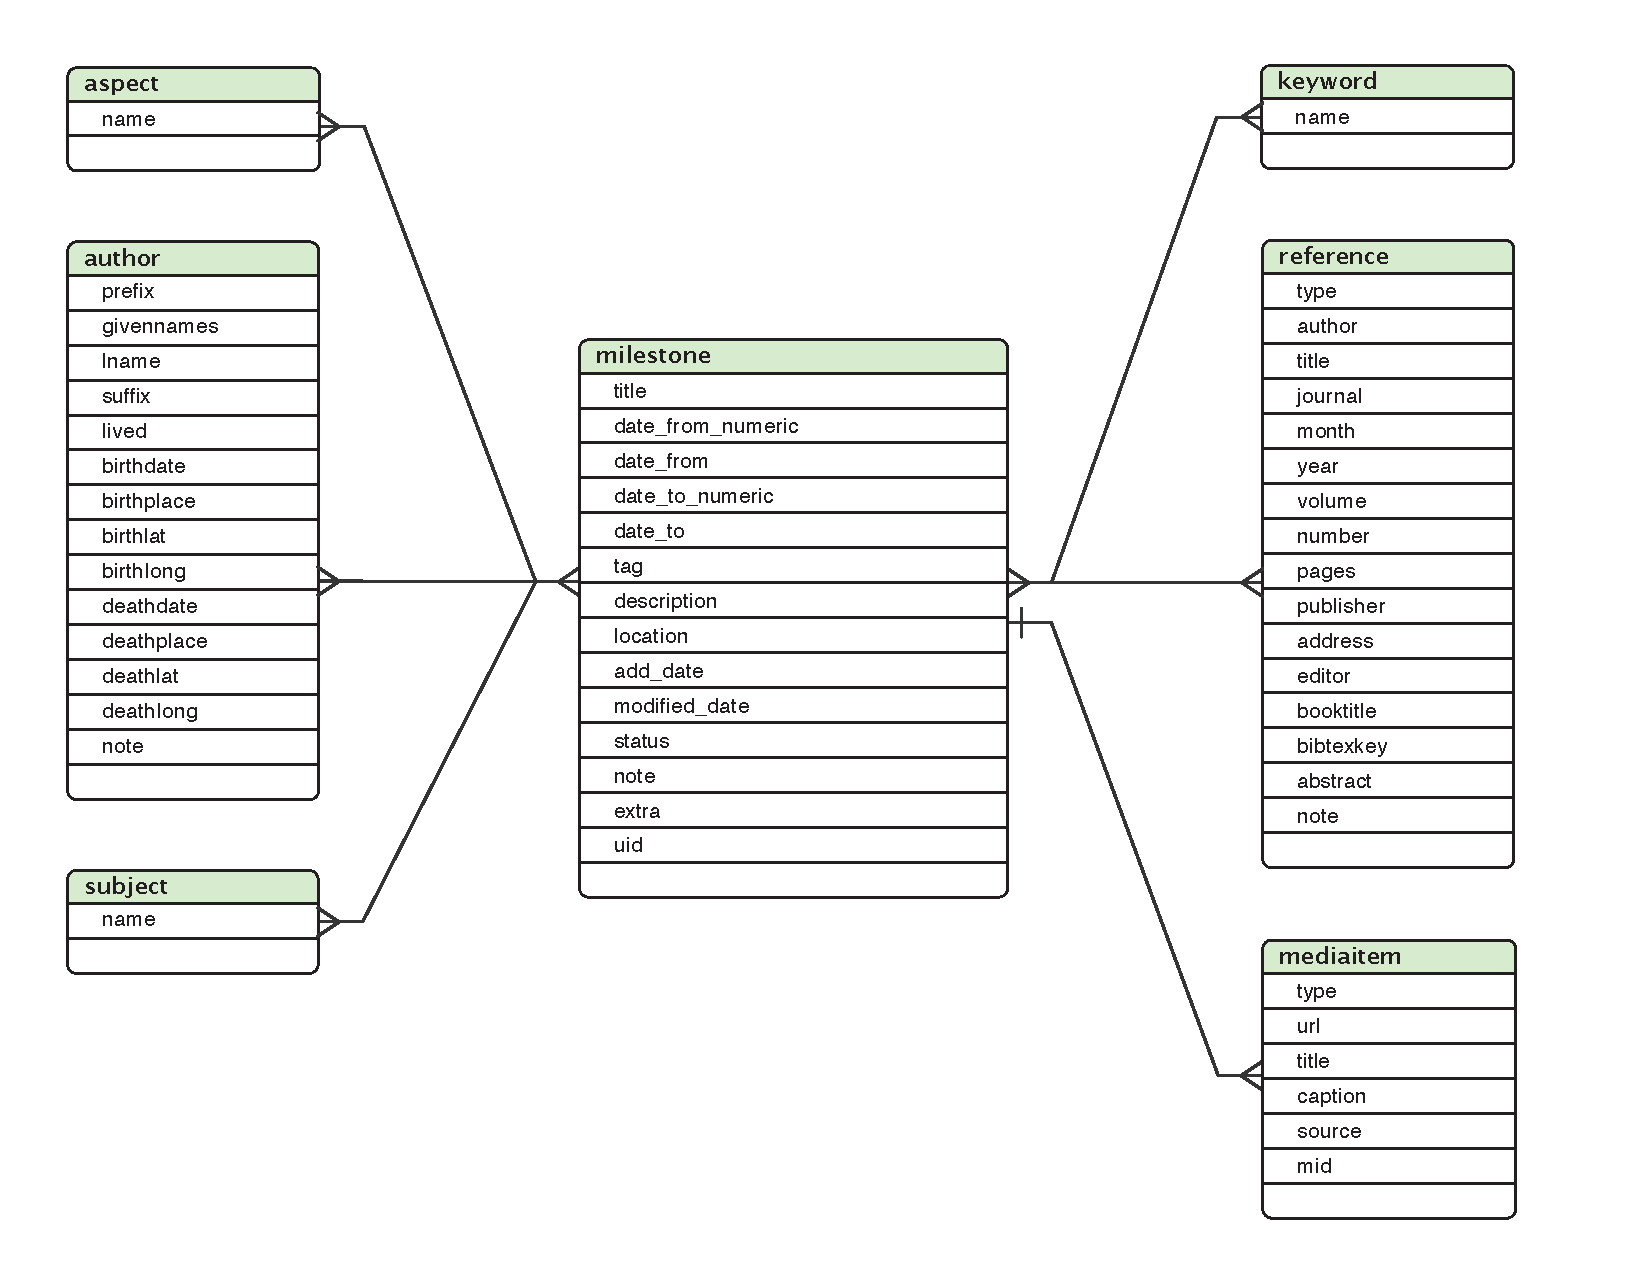
\includegraphics[width=\textwidth,clip]{fig/datavis-db-schema-reduced}
  \caption{Simplified schema for the MySQL database for the Milestones Project. The main 
  table (\texttt{milestone}) contains information regarding each of the items considered
  a milestone in the history of data visualization, linked to other tables 
  (e.g., \texttt{reference}, \texttt{mediaitem}) by unique keys.
  Other supporting tables, not shown here, provide for convenient lookup of 
  descriptors of these milestones items (\texttt{subject}, \texttt{aspect}, \texttt{keyword}).
  }
  \label{fig:datavis-db-schema}
\end{figure}


At present, the Milestones Project lists 288 contributions to this history, with nearly 350 references,
information on 336 authors and 774 ``media items'', comprising 371 images appearing online on the
\url{http://datavis.ca} site and 403 links to images and documents at other sites.
In addition, we maintain an offline image database comprising over 1100 images collected from
various sources, ...

\figref{fig:datavis-timeline2} shows the timeline view of the miletsones items displayed on the
landing page. ...

